\documentclass[a4paper]{ctexart}
\usepackage[top=2.3cm,bottom=2cm,left=1.7cm,right=1.7cm]{geometry} 
\usepackage{amsmath, amssymb}
\usepackage{color}
\usepackage{listings}
\usepackage{mathrsfs} 
\usepackage{booktabs}
\usepackage{amsthm}
\usepackage{longtable} 
\usepackage{graphicx}
\usepackage{subfigure}
\usepackage{caption}
\usepackage{fontspec}
\usepackage{titlesec}
\usepackage{fancyhdr}
\usepackage{latexsym}
\usepackage{subfigure}
\usepackage{cite}
\CTEXsetup[format={\Large\bfseries}]{section}
\def\d{\mathrm{d}}
\def\e{\mathrm{e}}
\newcommand{\mb}[1]{\mathbf{#1}}
\newcommand{\mr}[1]{\mathrm{#1}}
\newcommand{\dv}[2]{\frac{\d{#1}}{\d{#2}}}
\newcommand{\pdv}[2]{\frac{\partial{#1}}{\partial{#2}}}
\def\degree{$^{\circ}$}
\title{\textbf{鼓的振动模态}}
\author{}
\date{}
% 注意,重新定义了微分与偏微分的表达,使之更加简洁
\makeatletter %使\section中的内容左对齐
\makeatother
\begin{document}
	\pagestyle{fancy}
	\pagestyle{fancy}
    \lhead{音乐与数学期末课题}
	\chead{}
	\rhead{\today}
	\maketitle
	\thispagestyle{fancy}
	\section{鼓与振动}
	\subsection{鼓的构造}
	鼓是一种由近似圆柱形的鼓身和鼓身一端或两端蒙上拉紧的膜构成的打击乐器。
	演奏时通常是演奏者击打圆形的鼓面,鼓面振动发出声音,可以将发声过程看作
	圆形薄膜的振动过程。但是真实的鼓发声过程并不简单地对应于一个边界固定的
	圆形薄膜的自由振动(没有耗散,没有外力),比如我们忽略了鼓面的能量耗散:
	鼓面与空气的相互作用,鼓面本身的阻尼等等。想要建立准确的符合实际的模型,
	首先需要在物理上对鼓进行分类。
	\par 鼓作为振动系统可以分为3类\cite{a}:
	1.由单个薄膜与封闭的空气室构成(kettledrums),2.由单个薄膜和两侧均开放的空气室构成(tom-toms, congas),
	3.由两片薄膜与中间封闭的空气室耦合而成(bass drums, snare drums)。可以看到,
	真实的情况远比理想的薄膜振动要复杂,不仅涉及到鼓面与空气作用导致的能量耗散,甚至
	涉及到两个鼓面振动的耦合。
	\subsection{膜自由振动波动方程的建立}
	要想精确描述一个振动过程,必须找到与之对应的波动方程。但是真实的情况非常复杂,
	只能先从理想的情况开始讨论。
	我们\textbf{假设}膜上的每一点都在垂直于薄膜平面(平衡位置)的方向上做小振动,
	这样用一个标量可以完全描述每一点的运动情况,得到的波动方程是标量波动方程。
	用坐标$(x, y)$来标记平衡时每一点的位置,用$u(x, y)$来标记与平衡位置的偏离。
	\textbf{假设}薄膜没有厚度,薄膜的形变不能带来法向的张力,
	即膜的内部只有平行于薄膜的张力(这个假设与柔软的弦是一样的),
	很显然这个假设对于平板(和细杆)是不成立的,也就是说将要得到的波动方程
	并不能描述与它们的振动。
	\par 建立波动方程的思路是考虑一小块薄膜的受力情况,写出它对应的运动方程。如图(\ref{force})
	所示,OABC表示偏离平衡位置的薄膜,O点的坐标为$(x, y)$。假设这个薄膜的应力张量
	为$\sigma$,在最一般的情况下也是位置与时间的函数。
	\begin{figure}[htbp]
		\centering
		\includegraphics[scale=0.2]{force.png}
		\caption{薄膜微元的受力分析}
		\label{force}
	\end{figure} 
	可以通过应力张量表示出这个小薄膜的每个边的受力情况:
	\begin{align}
		F_{\mr{AB}, x} &= \int_{\mr{A}}^{\mr{B}} \sigma_{xy}\d x + \sigma_{xx}\d y \approx \sigma_{xx}(x+\Delta x, y)\Delta y\\
		F_{\mr{AB}, y} &= \int_{\mr{A}}^{\mr{B}} \sigma_{yy}\d x + \sigma_{yx}\d y \approx \sigma_{yx}(x+\Delta x, y)\Delta y\\
		F_{\mr{OC}, x} &= \int_{\mr{O}}^{\mr{C}} \sigma_{xy}\d x + \sigma_{xx}\d y \approx \sigma_{xx}(x, y)\Delta y\\
		F_{\mr{OC}, y} &= \int_{\mr{O}}^{\mr{C}} \sigma_{yy}\d x + \sigma_{yx}\d y \approx \sigma_{yx}(x, y)\Delta y\\
		F_{\mr{OA}, x} &= \int_{\mr{O}}^{\mr{A}} \sigma_{xy}\d x + \sigma_{xx}\d y \approx \sigma_{xy}(x, y)\Delta x\\
		F_{\mr{OA}, y} &= \int_{\mr{O}}^{\mr{A}} \sigma_{yy}\d x + \sigma_{yx}\d y \approx \sigma_{yy}(x, y)\Delta x\\
		F_{\mr{CB}, x} &= \int_{\mr{C}}^{\mr{B}} \sigma_{xy}\d x + \sigma_{xx}\d y \approx \sigma_{xy}(x, y + \Delta y)\Delta x\\
		F_{\mr{CB}, y} &= \int_{\mr{C}}^{\mr{B}} \sigma_{yy}\d x + \sigma_{yx}\d y \approx \sigma_{yy}(x, y + \Delta y)\Delta x
	\end{align}
	\par 上面的约等于在薄膜很小的情况下成立,忽略了一些在后面计算二阶导数时可以忽略的高阶小量。
	下面将计算每个边的受力在$z$方向上的分量(因为我们假设只在$z$方向上有运动),
	\textbf{假设}薄膜只做微小的振动,在这种情况下,$x$方向的力在$z$方向的贡献可以用
	薄膜沿$x$方向的切线与$x$轴夹角的正切值,也就是$\pdv{u}{x}$来衡量;同样的,$y$方向的
	力对$z$方向的力的贡献可以用$\pdv{u}{y}$来衡量。那么AB,\, CO两个边对于$z$方向的力的
	贡献为:
	\begin{align}
		F_{1} =& \,\sigma_{xx}(x+\Delta x, y)\Delta y\pdv{u}{x}(x+\Delta x, y) + \sigma_{yx}(x+\Delta x, y)\Delta y\pdv{u}{y}(x+\Delta x, y)\\
		&- \sigma_{xx}(x, y)\Delta y\pdv{u}{x}(x, y) + \sigma_{yx}(x, y)\Delta y\pdv{u}{y}(x, y)\\
		\approx& \, \left[\pdv{}{x}\left(\sigma_{xx}\pdv{u}{x}\right) + \pdv{}{x}\left(\sigma_{yx}\pdv{u}{y}\right)\right]\Delta x\Delta y
	\end{align}
	\par 同理OA,\, CB两个边对于$z$方向力的贡献为:
	\begin{align}
		F_{2} \approx  \left[\pdv{}{y}\left(\sigma_{xy}\pdv{u}{x}\right) + \pdv{}{y}\left(\sigma_{yy}\pdv{u}{y}\right)\right]\Delta x\Delta y
	\end{align}
	\par 那么,根据Newton运动定律,薄膜微元的振动方程可以写为:
	\begin{align}
		&F_{1} + F_{2} = \rho \Delta x\Delta y \pdv{^{2}u}{t^{2}}\\
		\Rightarrow& \left[\pdv{}{x}\left(\sigma_{xx}\pdv{u}{x}\right) + \pdv{}{x}\left(\sigma_{yx}\pdv{u}{y}\right)\right] + 
		\left[\pdv{}{y}\left(\sigma_{xy}\pdv{u}{x}\right) + \pdv{}{y}\left(\sigma_{yy}\pdv{u}{y}\right)\right] = \rho\pdv{^2 u}{t^{2}}
	\end{align}
	\par 这是一般的没有能量耗散的薄膜小振动时所满足的方程,其中应力张量可以是位置
	和时间的函数,在小振动假设下,一般认为其只是位置的函数。考虑到应力张量总是一
	个对称张量\cite{b},可以将上面的波动方程表示为一个更加紧凑的形式,其中使用了求和约定:
	\begin{align}
		\pdv{}{x^{i}}\left(\sigma_{ij}\pdv{u}{x^{j}}\right) = \rho\pdv{^2 u}{t^2}
	\end{align}
	
	进一步\textbf{假设}薄膜在平衡时内部的应力张量是一个常量(与位置无关,比如在各个
	方向均匀地拉伸一个各向同性方形薄膜),同时考虑到这是一个对称张量,那么可以选取
	一个特殊的直角坐标系使得每一点处的张量都具有对角的形式,方程可以化简为:
	\begin{align}
		\sigma_{xx}\pdv{^{2}u}{x^{2}} + \sigma_{yy}\pdv{^2 u}{y^2} = \rho \pdv{^{2}u}{t^{2}}
	\end{align}
	\par 如果进一步假设薄膜是各向同性的,应力张量为一个常数乘上单位张量
	那么薄膜的小振动方程在任意一个直角坐标系下都可以写成:
	\begin{align}
		\pdv{^2 u}{x^2} + \pdv{^{2}u}{y^{2}} = \frac{1}{c^{2}}\pdv{^2 u}{t^2}\quad\quad\quad c^2 = \frac{\sigma}{\rho}
		\label{wave eq}
	\end{align}
	\par 其中$c$称为波速。将要求解的就是这个波动方程,这是一个理想化的模型,我们做了足够多的假设。
	\section{固定边界的圆膜的振动}
	\subsection{问题的描述}
	由于鼓面的四周是完全固定的,在考虑初始条件后可以构成一个定解问题。假设
	圆膜的半径为$a$,给定初始时刻时圆膜上每一点的位移和速度,定解问题可以写为:
	\begin{align}
		\left\{
			\begin{array}{lr}
				\displaystyle\frac{1}{c^2}\pdv{^{2}u}{t^2} = \nabla^{2}u\\
				\displaystyle u|_{x^2 + y^2 = a^2} = 0\\
				\displaystyle u|_{t=0} = f(x, y),\, \pdv{u}{t}|_{t=0} = g(x, y)
			\end{array}
		\right.
	\end{align}
	\par 由于求解区域的特殊性,考虑将方程转化到极坐标中,同时要转换方程与定解条件:
	\begin{align}
		\left\{
			\begin{array}{lr}
				\displaystyle\frac{1}{c^2}\pdv{^{2}u}{t^2} = \frac{1}{r}\pdv{}{r}\left(r\pdv{u}{r}\right) + \frac{1}{r^2}\pdv{^2 u}{\phi^{2}}\\
				\displaystyle u|_{\phi=0} = u|_{\phi=2\pi},\, \left.\pdv{u}{\phi}\right|_{\phi=0} = \left.\pdv{u}{\phi}\right|_{\phi=2\pi}\\
				\displaystyle u|_{r=0}\,\,\mr{finit},\, u|_{r=a}=0\\
				\displaystyle u|_{t=0} = F(r, \phi),\, \left.\pdv{u}{t}\right|_{t=0} = G(r, \phi)
			\end{array}
			\label{wave eq of drum}
		\right.
	\end{align}
	\par 将直角坐标转换成极坐标时,人为地增添了一些边界条件,这些边界条
	件在物理上很好理解:首先在直角坐标系中原点并不是奇点,因此转换为极坐标后
	也得要求原点的解不能发散(不是奇点);其次解应该是角度的周期函数,
	因为转过$2\pi$角度回到圆膜上同一个点,振动情况完全相同。
	\par 也可以给出数学角度的理解:直角坐标与极坐标之间的变换将一个圆形
	和一个长方形对应,
	但是这个“对应”的性质不总是很好,首先圆心处映射并不是单射,圆心对应于
	长方形的一个边;其次边界并不对应边界,圆形的边界对应于长方形的一个边,
	圆形区域内部的一条线(规定$\phi=0$的那条线)对应于长方形的两个边。
	这个映射破坏了原本圆形的拓扑,相当于挖去了圆心后再沿圆心处将圆形剪开,
	再把这个图形“连续地”映射成了一个长方形。在讨论区域上的函数时,
	区域的性质会影响其上函数的性质,最直接的就是影响连续性和可微性,上面的边界条件
	相当于将定义在矩形上的函数“沿着某个边粘起来”,使之可以定义在圆形的区域上。
	\par 将要求解的是转化到极坐标后,与原来问题等价的方程。
	\subsection{没有耗散的情形}
	上面导出的方程对应于没有耗散的情形,希望能够通过求解方程给出固定边界
	圆膜振动的普遍描述。首先假设方程具有满足$r\, \phi$方向
	边界条件(不一定满足初始条件)的分离变量形式的特解:
	\begin{align}
		u(r, \phi, t) = v(r, \phi)T(t)
	\end{align}
	\par 将所有分离变量形式的解\textbf{线性组合}使其满足\textbf{初始条件}
	就可以得到定解问题的解。将这样的解代入方程并分离变量:
	\begin{align}
		\frac{1}{c^2}\frac{T''(t)}{T} = \frac{1}{rv(r,\phi)}\pdv{}{r}\left(r\pdv{v}{r}\right)
		 + \frac{1}{r^2 v(r,\phi)}\pdv{^2 v}{\phi^2}
	\end{align}
	\par 方程两边没有相同的自变量,因此只能等于同一个常数,
	令其为$-\lambda$,得到两个常微分方程:
	\begin{align}
		T{''}(t) + \lambda c^2T(t) = 0
		\label{time eq}
	\end{align}
	\begin{align}
		\frac{1}{r}\pdv{}{r}\left(r\pdv{v}{r}\right) + \frac{1}{r^2}\pdv{^2 v}{\phi^2} + \lambda v = 0
		\label{mode}
	\end{align}
	\par 其中$v$满足的$r, \phi$方向上的边界条件与$u$的相同,共同构成一个偏微
	分方程本征值问题,求解出所有本征值$\lambda$与本征函数并与对应的时间
	方程的解组合就得到圆膜振动的一个特解,考虑到本征函数的完备性,这些解的
	线性组合可以构成满足任意初始条件的解,因此研究这个偏微分方程的本征值
	问题与对应的分离变量的解的性质对于研究圆膜振动有着重要的意义。
	\par 为了求解偏微分方程本征值问题,进一步考虑$v$也有分离变量形式
	的满足边界条件的解$v(r, \phi) = R(r)\Phi(\phi)$,带入方程分离变量得到:
	\begin{align}
		\frac{r}{R}\dv{}{r}\left(r\dv{R}{r}\right) + \lambda r^{2} = -\frac{1}{\Phi}\dv{^2 \Phi}{\phi^2} = \mu
	\end{align}
	\par 通过$v(r, \phi)$满足的边界条件得到$R(r), \Phi(\phi)$满足的边界条件(直接带入):
	\begin{align}
		&\left\{
			\begin{array}{lr}
				R(r)\Phi(0) = R(r)\Phi(2\pi)\\
				R(r)\Phi'(0) = R(r)\Phi'(2\pi)
			\end{array}
		\right.\\
		&\left\{ 
			\begin{array}{lr}
				R(0)\Phi(\phi)\quad \mr{finit}\\
				R(0)\Phi(\phi) = 0
			\end{array}
		\right.
	\end{align}
	\par 考虑到$R,\, \Phi$均不恒等于0(否则只能给出0解),
	这些边界条件与分离变量产生的两个微分方程构成了常微分方程本征值问题:
	\begin{equation}
		\left\{ 
			\begin{array}{lr}
				\displaystyle\frac{1}{r}\dv{}{r}\left(r\dv{R}{r} \right) + \left(\lambda - \frac{\mu}{r^2}\right)R = 0\\
				R(0)\quad\mr{finit}\\
				R(a) = 0
			\end{array}
		\right.
		\label{non_reduced Bessel equation}
	\end{equation}
	\begin{equation}
		\left\{ 
			\begin{array}{lr}
				\displaystyle\dv{^2\Phi}{\phi^2} + \mu \Phi = 0\\
				\Phi(0) = \Phi(2\pi)\\
				\Phi'(0) = \Phi'(2\pi)
			\end{array}
		\right.
		\label{angle equation}
	\end{equation}
	\par 本征值问题(\ref{angle equation})的解这里不仔细求解(容易写出方程的通解,
	仔细讨论满足边界条件的非平凡解就可以得到本征值和本征函数),直接给出结论(
	可以参考\cite{mathematicalmethod}第15章第4节):
	\begin{align}
		\left\{ 
			\begin{array}{lr}
				\mu = m^{2}\\
				\Phi_{m1} = \sin(m\phi)\\
				\Phi_{m2} = \cos(m\phi)\\
				m = 0,1,2,\cdots 
			\end{array}
		\right.
	\end{align}
	\par 这里注意一下对于同一个本征值$m^2 \neq 0$对应两个简并的本征函数;但当$m^2=0$时,
	仅对应一个本征函数$\Phi_{02} = 1$。
	\par 对于本征值问题(\ref{non_reduced Bessel equation}),首先将其转化为标准形式,
	令$x = \sqrt{\lambda}r,\, y = R(r)$:
	\begin{align}
		\left\{ 
			\begin{array}{lr}
				\displaystyle\frac{1}{x}\dv{}{x}\left(x\dv{y}{x} \right) + \left(1 - \frac{m^2}{x^2}\right)y = 0\\
				y(0)\quad\mr{finit}\\
				y(\sqrt{\lambda}a) = 0\\
				m = 0, 1, 2, \cdots
			\end{array}
		\right.
	\end{align}
	\par 
	这是一个整数阶Bessel方程,其通解可以写为(参考\cite{mathematicalmethod}
	第17章第1节):
	\begin{align}
		y(x) = AJ_{m}(x) + BN_{m}(x)
	\end{align}
	\par 其中$J_{m}(x),\,N_{m}(x)$为m阶Bessel函数与m阶Neumann函数。由于整数阶Neumann
	函数在0处发散,为了满足$x=0$处函数值有界的边界条件,只能要求$B=0$。
	带入另一个边界条件可以得到:
	\begin{align}
		J_{m}(\sqrt{\lambda}a) = 0
	\end{align}
	\par 这意味着需要知道Bessel函数的零点进而得到可取的$\lambda$值(本征值),用
	$\mu_{i}^{(m)}$表示m阶Bessel函数的零点(i是对于不同零点的一个标记),$\lambda$
	满足的条件为:
	\begin{align}
		\sqrt{\lambda} a = \mu_{i}^{(m)}
		\Rightarrow \lambda = \left(\frac{\mu_{i}^{(m)}}{a}\right)^2 
	\end{align}
	\par 可以证明Bessel函数的零点均对称分布在实轴上\cite{specialfunction},
	对于整数阶Bessel函数,由于其具有奇偶性\cite{mathematicalmethod}:$J_n(-x) = (-1)^n J_n(x)$
	因此正根和负根给出线性相关的本征函数,不妨只考虑正根(如果考虑0为Bessel方程
	的根即$\lambda = 0$的情况,会使得本征函数整体为0,舍去),每一个本征值
	$\lambda_{mi} = \left(\frac{\mu_{i}^{(m)}}{a}\right)^2$对应一个
	本征函数。
	\par
	至此我们得到了本征值问题(\ref{non_reduced Bessel equation})的解:
	\begin{equation}
		\left\{ 
		\begin{split}
			\lambda_{mi} &= \left(\frac{\mu_{i}^{(m)}}{a}\right)^2\\
			R_{mi} &= J_{m}\left(\frac{\mu_{i}^{(m)}r}{a}\right)\\
			i &= 1, 2, 3,\cdots\\
		\end{split}
		\right.
	\end{equation}
	\par  其中$\mu_{i}^{(m)}$为m阶Bessel函数的第i个正零点。与角向方程
	的本征值问题[\ref{angle equation}]的解组合后可以构成偏微分方程
	本征值问题(\ref{mode})的解:
	\begin{equation}
		\left\{
		\begin{split}
			\lambda_{mi} &= \left(\frac{\mu_{i}^{(m)}}{a}\right)^2\\
			v_{1mi} &= J_m\left(\frac{\mu_{i}^{(m)}r}{a}\right)\sin(m\phi)\\
			v_{1mi} &= J_m\left(\frac{\mu_{i}^{(m)}r}{a}\right)\cos(m\phi)\\
			m &= 0,1,2,\cdots\quad \quad i = 1, 2, 3,\cdots
		\end{split}
		\right.
	\end{equation}
	需要注意的是当$m=0$时,包含正弦函数的本征函数恒等于零,因此并不是本征函数,$m=0$
	时本征值问题只有包含余弦函数的那一个解,但是为了表述方便,所以采用了上面的写法。
	\par 
	在得到$\lambda$的取值后,可带入时间的方程(\ref{time eq})得到对应的$T(t)$
	的通解:
	\begin{align}
		T_{mi}(t) = A_{mi}\sin(\omega_{mi}t) + B_{mi}\cos(\omega_{mi}t)\quad \omega_{mi} = \frac{c\mu_{i}^{(m)}}{a}
	\end{align}
	\par 
	\par 与对应的$v_{mi}$组合后可得到波动方程的特解:
	\begin{equation}
		\left\{
			\begin{split}
				u_{1mi} &= \sin(\omega_{mi}t + \phi_{1mi}) 
				J_m\left(\frac{\mu_{i}^{(m)}r}{a}\right)\sin(m\phi)\\
				u_{2mi} &= \sin(\omega_{mi}t + \phi_{2mi})
				J_m\left(\frac{\mu_{i}^{(m)}r}{a}\right)\cos(m\phi)
			\end{split}
		\right.
		\label{vb mode}
	\end{equation}
	\par 
	仔细观察特解(\ref{vb mode})的特点,它表示圆膜上每一个点都以\textbf{相同的频率}$\omega_{mi} = \frac{c\mu_{i}^{(m)}}{a}$
	在平衡位置附近振动,振幅的分布用本征函数(\ref{mode})描述,其上有始终不振动的点称为\textbf{波节},
	也有振幅为极大值的\textbf{波腹},这样的波并不向远处传播而是在一定区域内以固定的模式振动,称其为
	\textbf{驻波},描述驻波的特解(\ref{vb mode})称为\textbf{驻波解},我们定义驻波解对应的振动模式
	为圆膜振动的\textbf{振动模态},使用本征值问题(\ref{mode})的指标$(m, i)$来标记每一个振动模态
	。由之前的讨论可知,定解问题(\ref{wave eq of drum})的解均可以表示为驻波解的线性组合:
	\begin{align}
		u(r, \phi, t) = \sum_{m=0}^{+\infty}\sum_{i=1}^{+\infty}(A_{mi}u_{1mi} + B_{mi}u_{2mi})
	\end{align}
	那么圆膜的任意一种振动可以等价地看作不同的振动模态以不同初相位相位振动的叠加(如果单独讨论一个振动模态,解中的相位没有绝对意义,但是讨论多个
	振动模态的叠加就要考虑振动的相位差)。因此,驻波解(振动模态)不但完备地描述了方程的解,而且具有清晰的物理图像。
	\subsection{振动模态的可视化} 
	\par 
	为了便于观察圆膜振动的具体行为,可以固定时间$t$,观察圆膜在三维空间中
	的形状。事实上由于正弦函数与余弦函数之间只相差相位,因此只用展示其中一种,
	将其旋转90\degree 后得到另一个与之简并的振动模态。
	图(\ref{vib img})\cite{mmtoffering}展示了对应于($n=0$只能采用$u_{20k}$)
	\begin{equation}
		u_{1nk} = \sin(\omega_{nk}t + \phi_{1nk}) 
				J_n\left(\frac{\mu_{k}^{(n)}r}{a}\right)\sin(n\phi)
	\end{equation}
	\begin{figure}[htbp]
		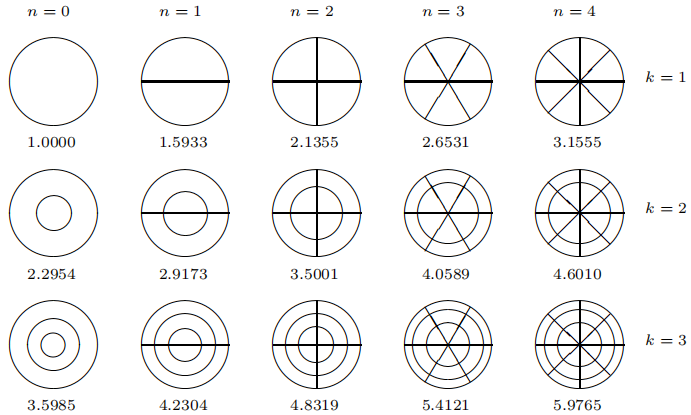
\includegraphics[scale=1]{vibration_mode_ideal.png}
		\centering
		\caption{理想圆膜振动模态的节点}
		\label{vib img}		
	\end{figure}
	的振动模态,其中实线对应于圆膜不发生振动的部分,即对应于驻波的节点,同时
	能够看出,随着振动模态的指标上升,节点数和分布有规律地增加,这是由Bessel函数与
	三角函数的性质决定的。
	\par 下面直接绘制出对应于余弦函数的振动模态(图(\ref{visual mode})):
	\begin{figure}[htbp]
		\begin{tabular}{ccccc}
			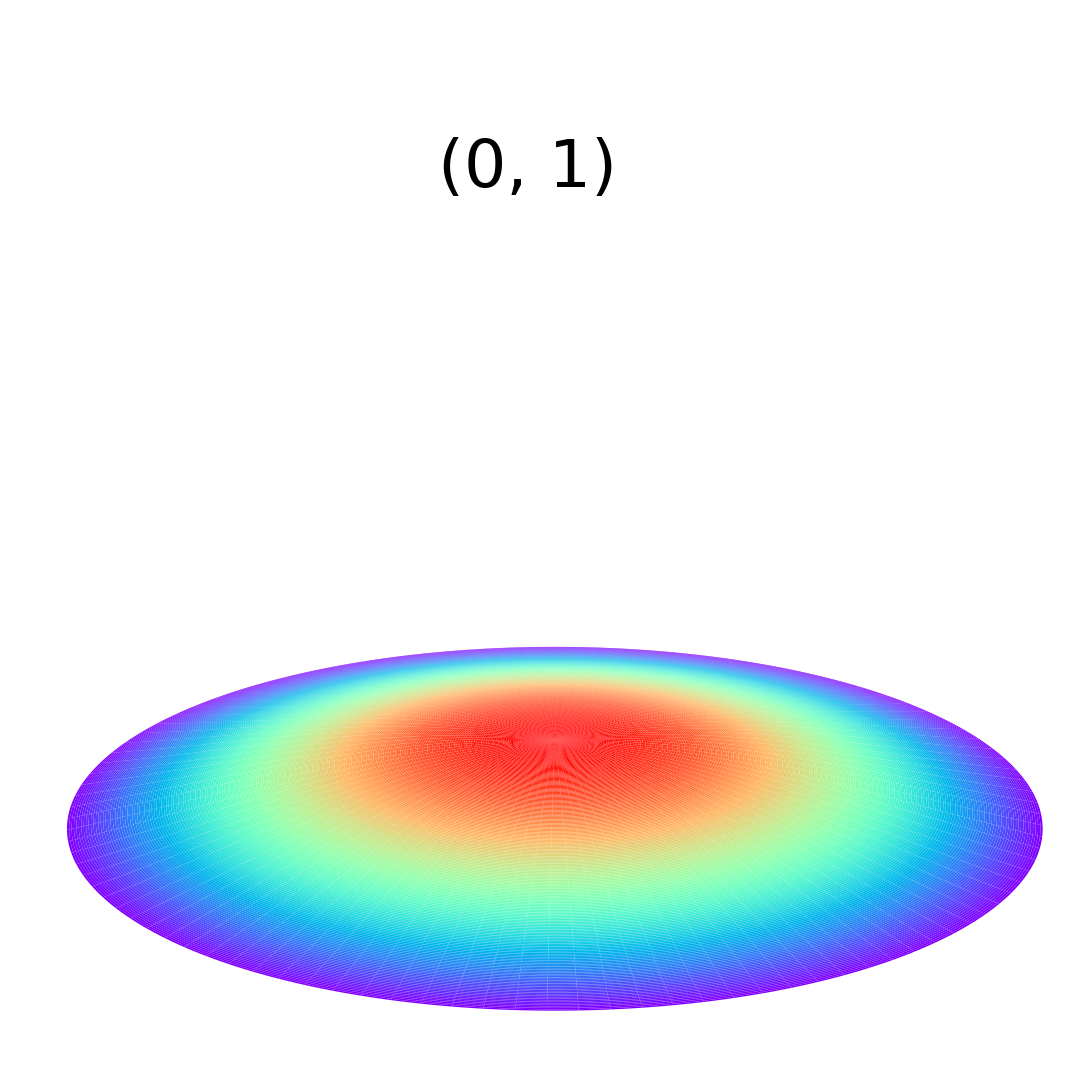
\includegraphics[scale=0.4]{0_1.png} & 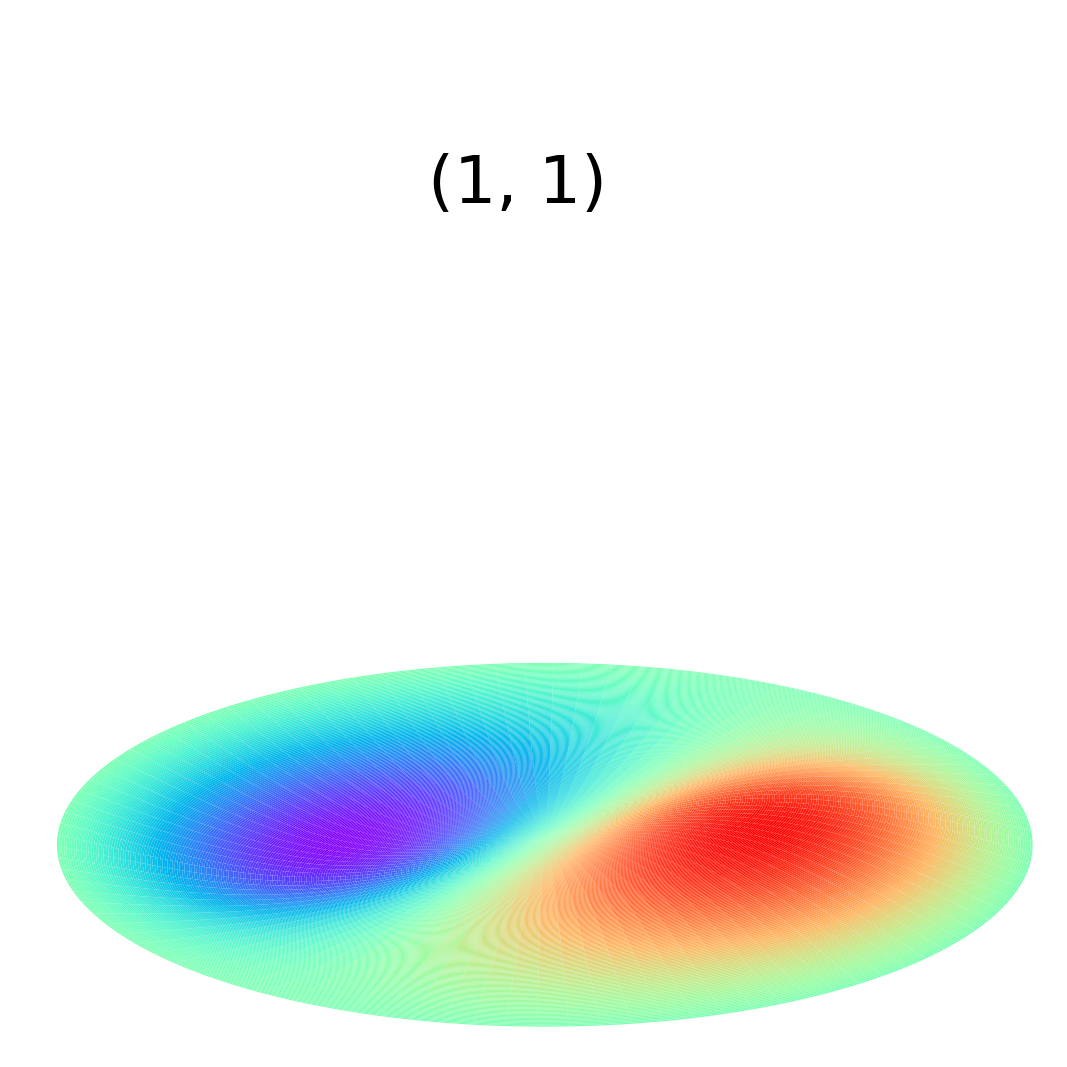
\includegraphics[scale=0.4]{1_1.png}
			& 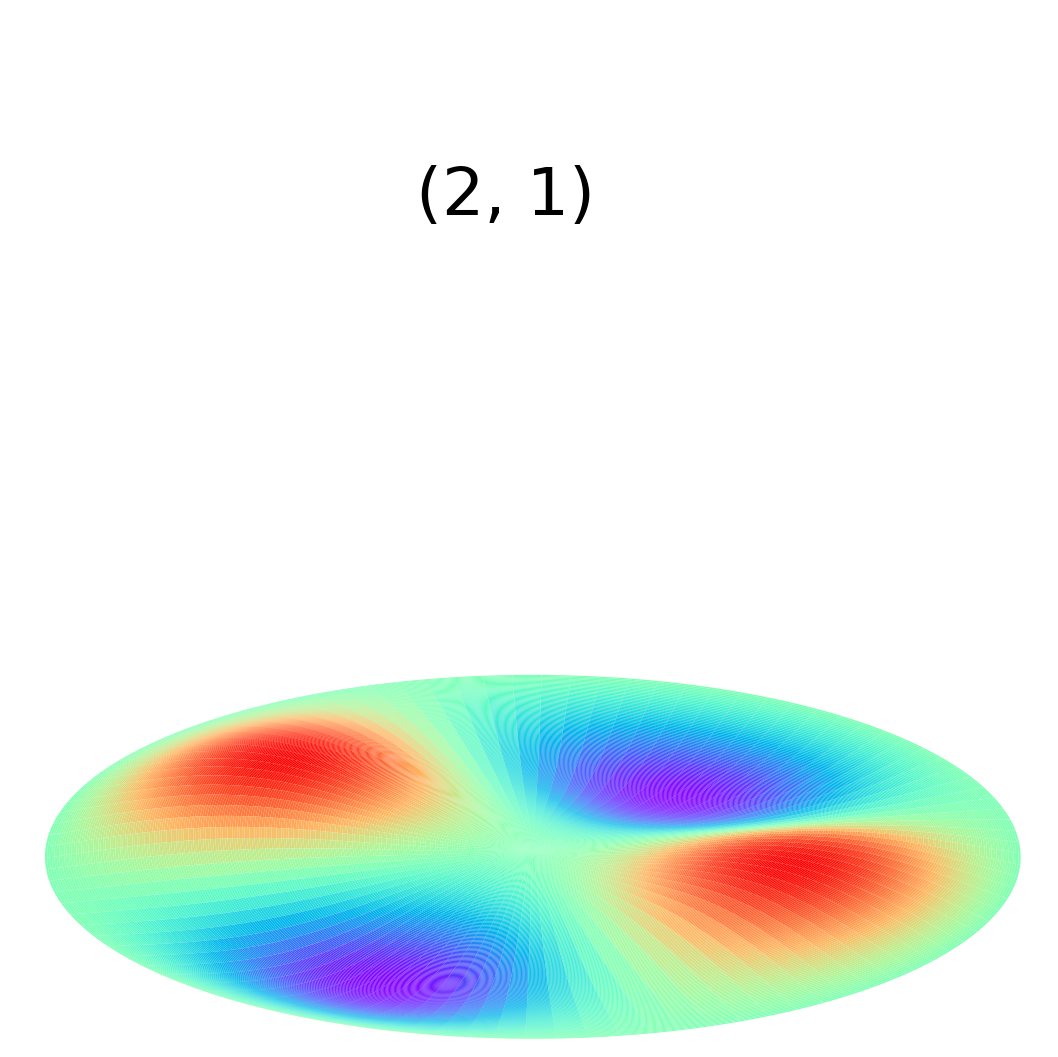
\includegraphics[scale=0.4]{2_1.png} & 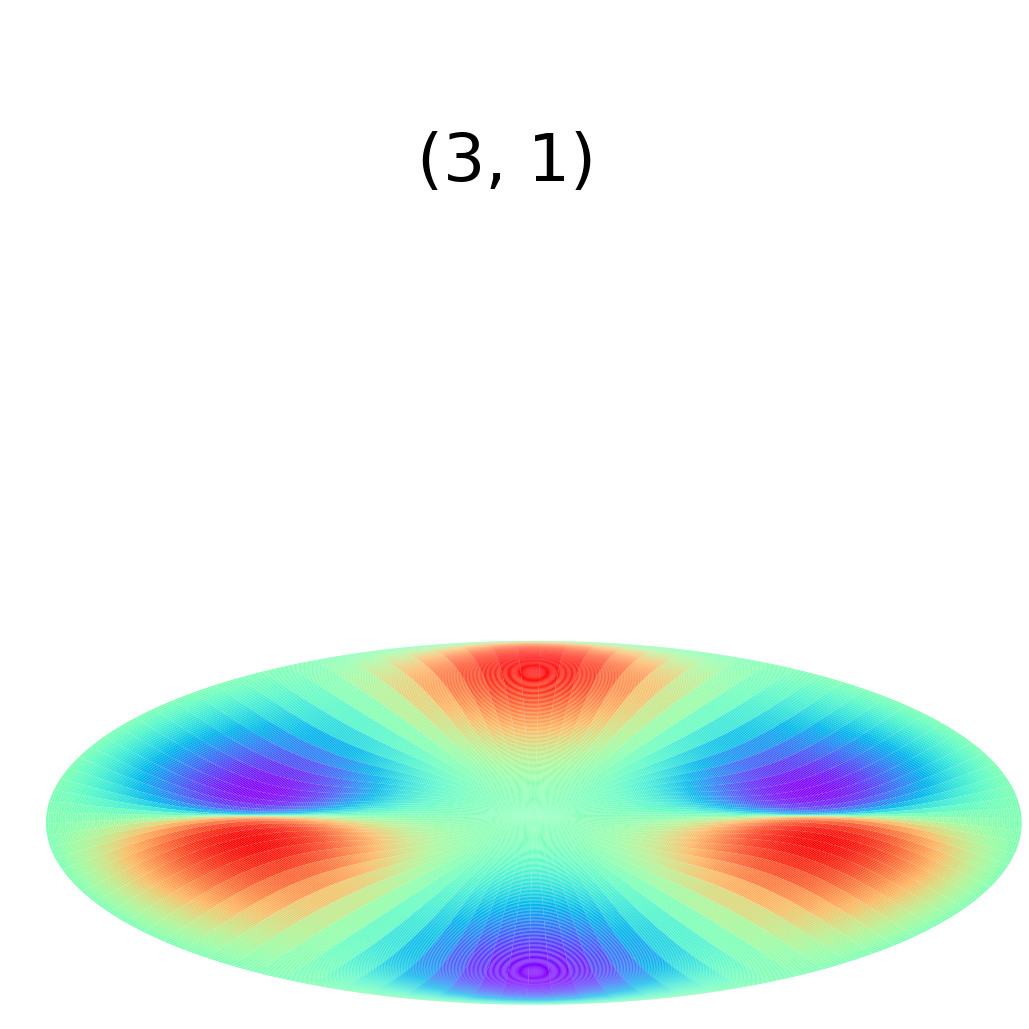
\includegraphics[scale=0.4]{3_1.png}
			& 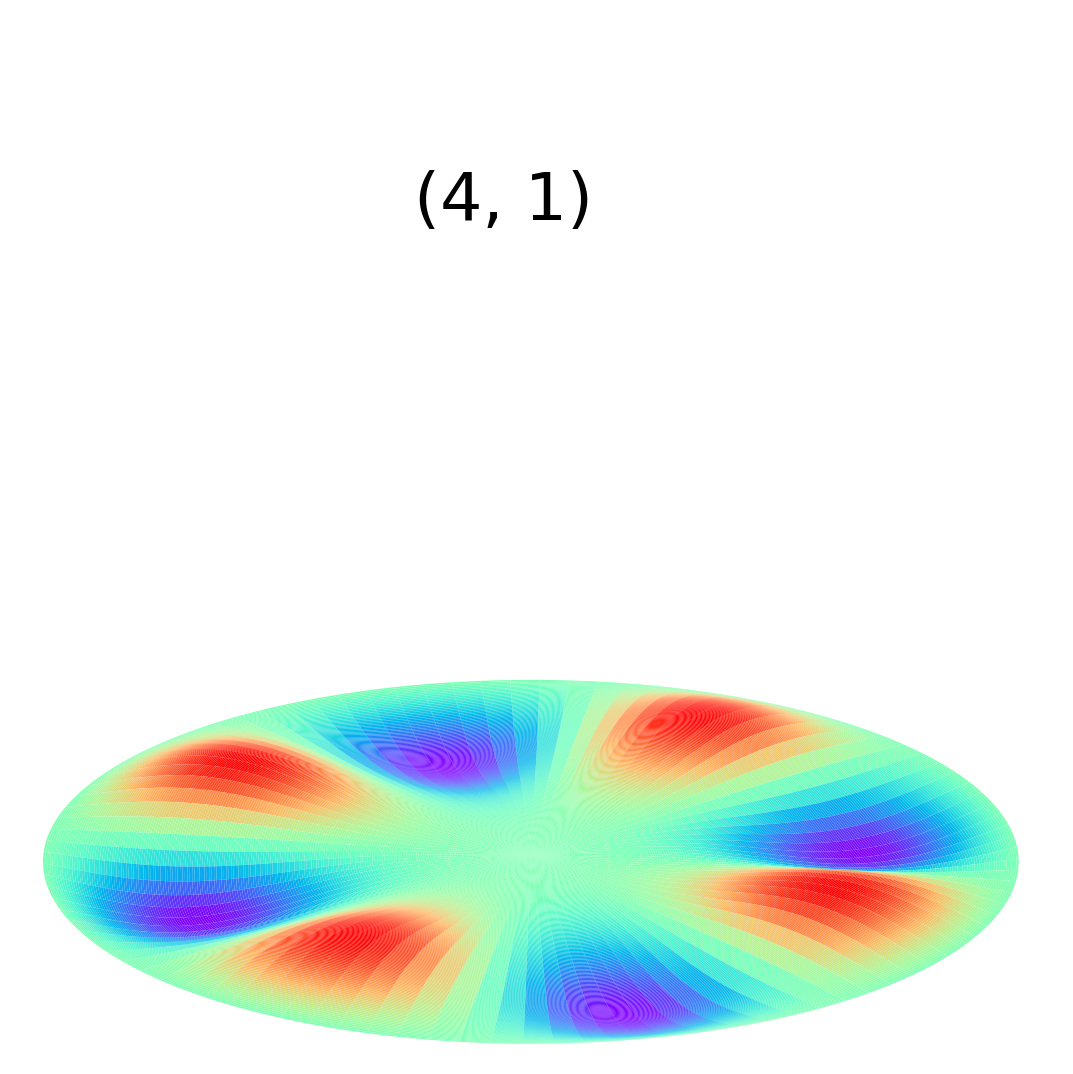
\includegraphics[scale=0.4]{4_1.png} \\
			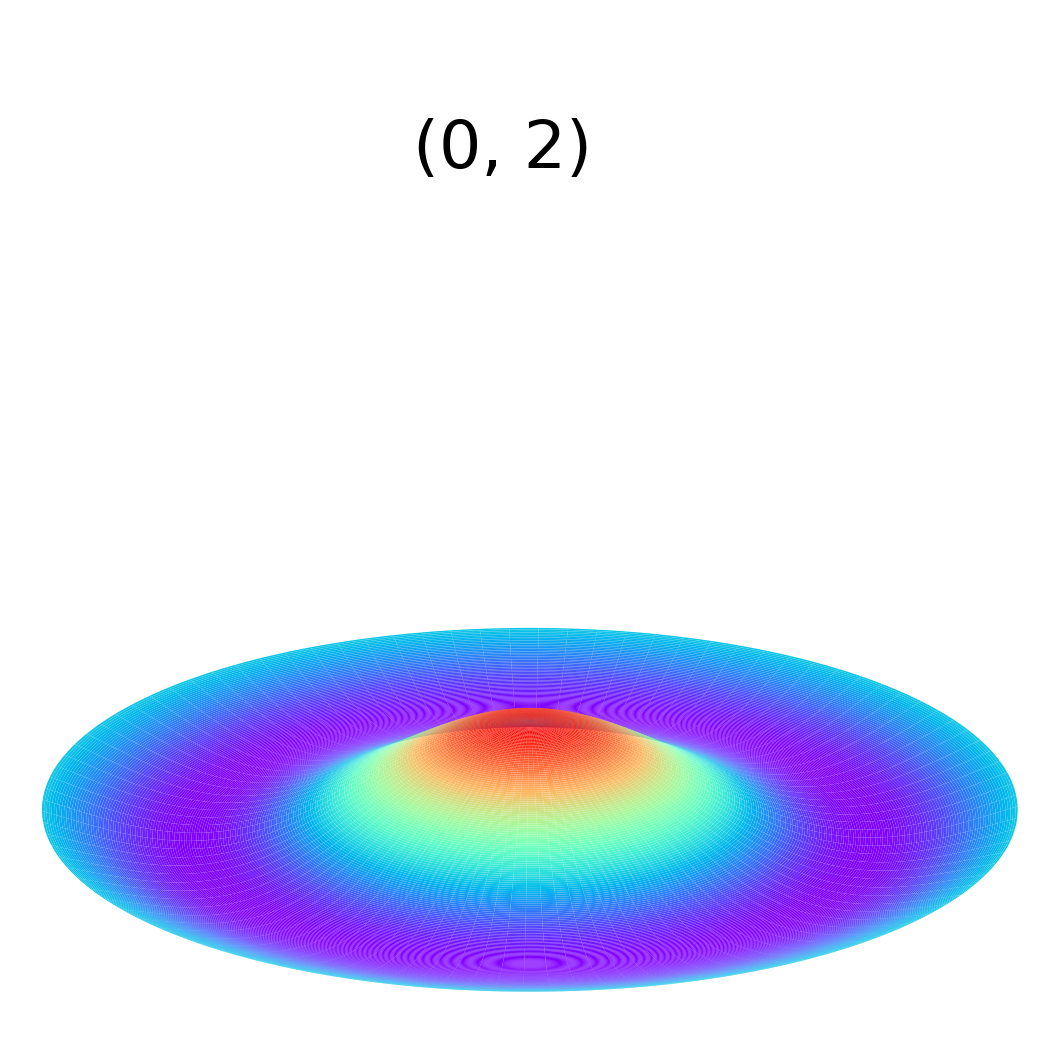
\includegraphics[scale=0.4]{0_2.png} & 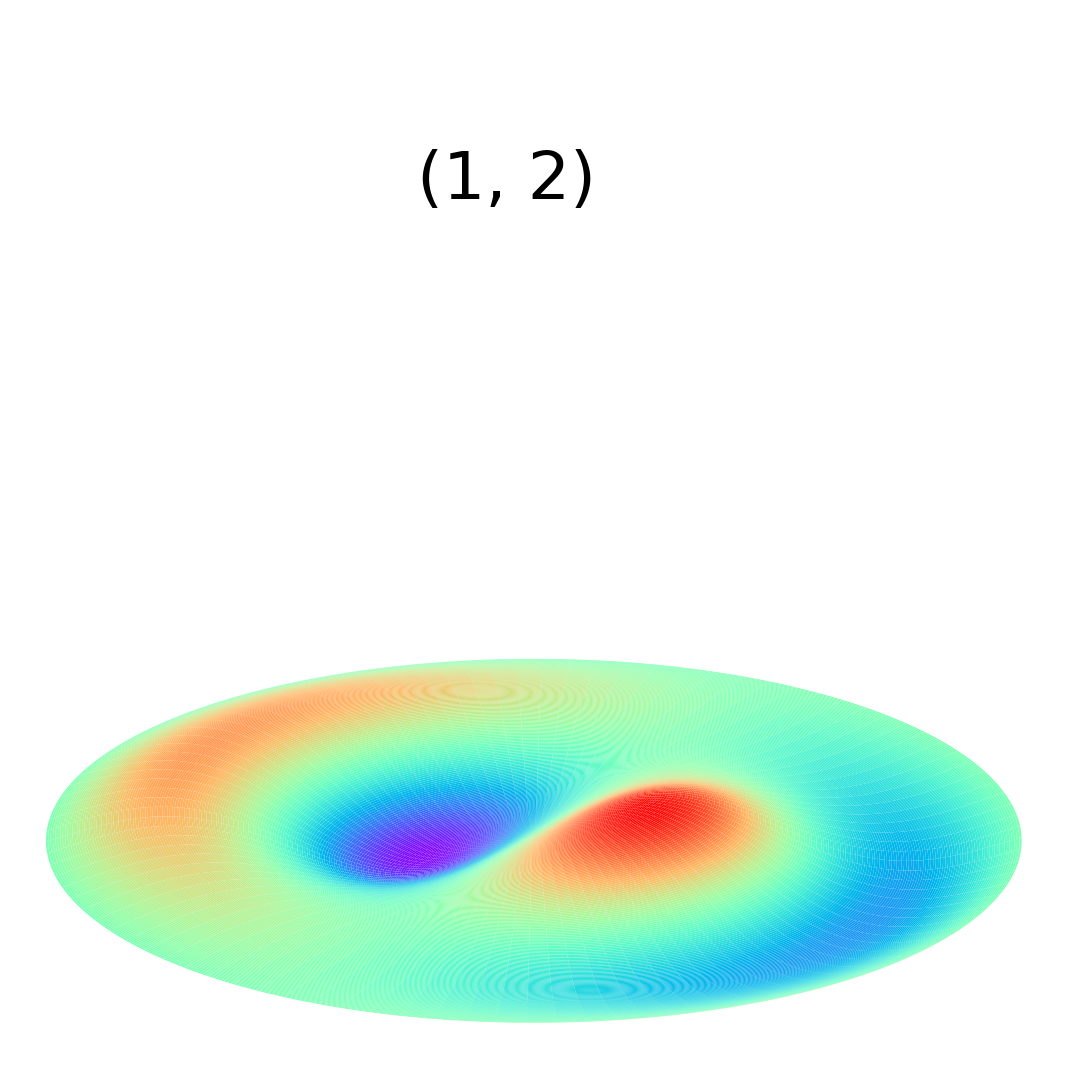
\includegraphics[scale=0.4]{1_2.png}
			& 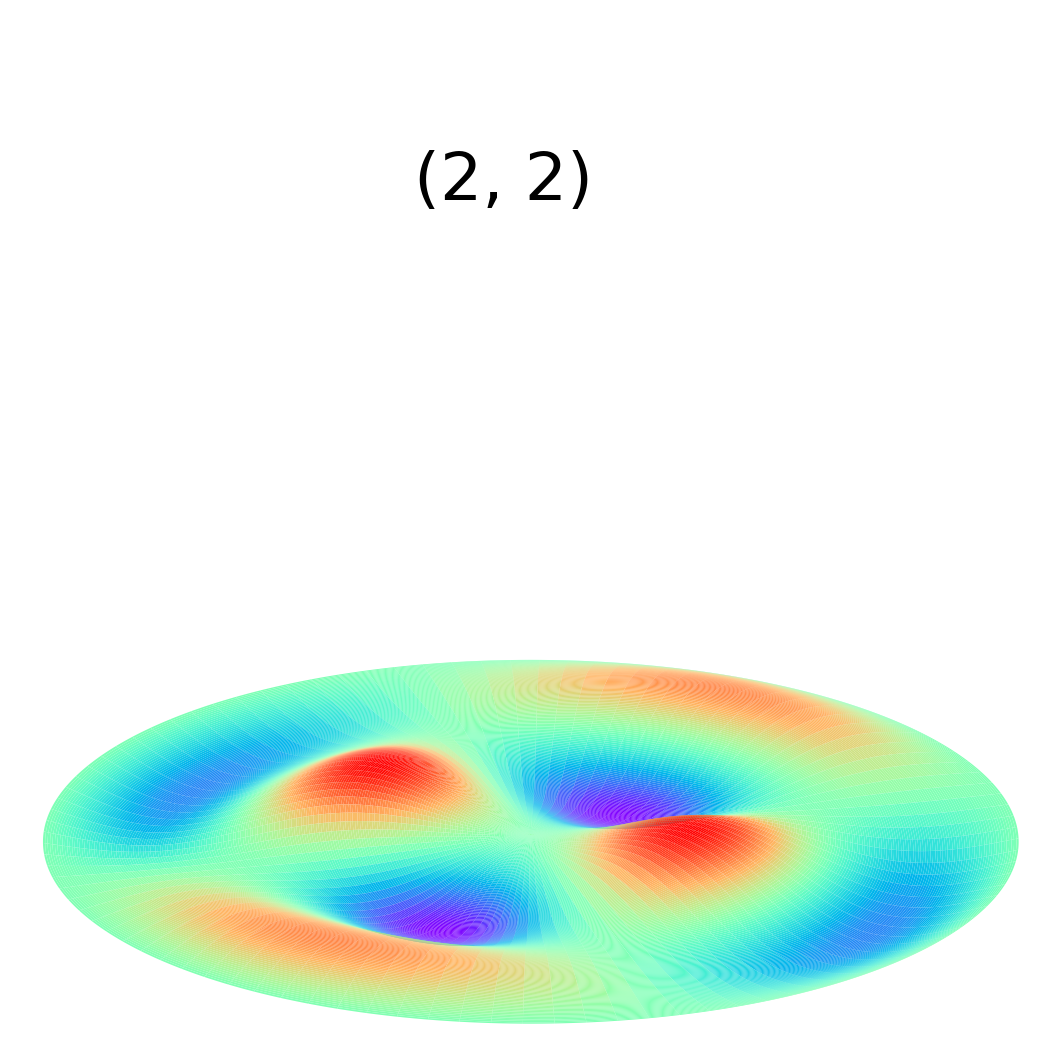
\includegraphics[scale=0.4]{2_2.png} & 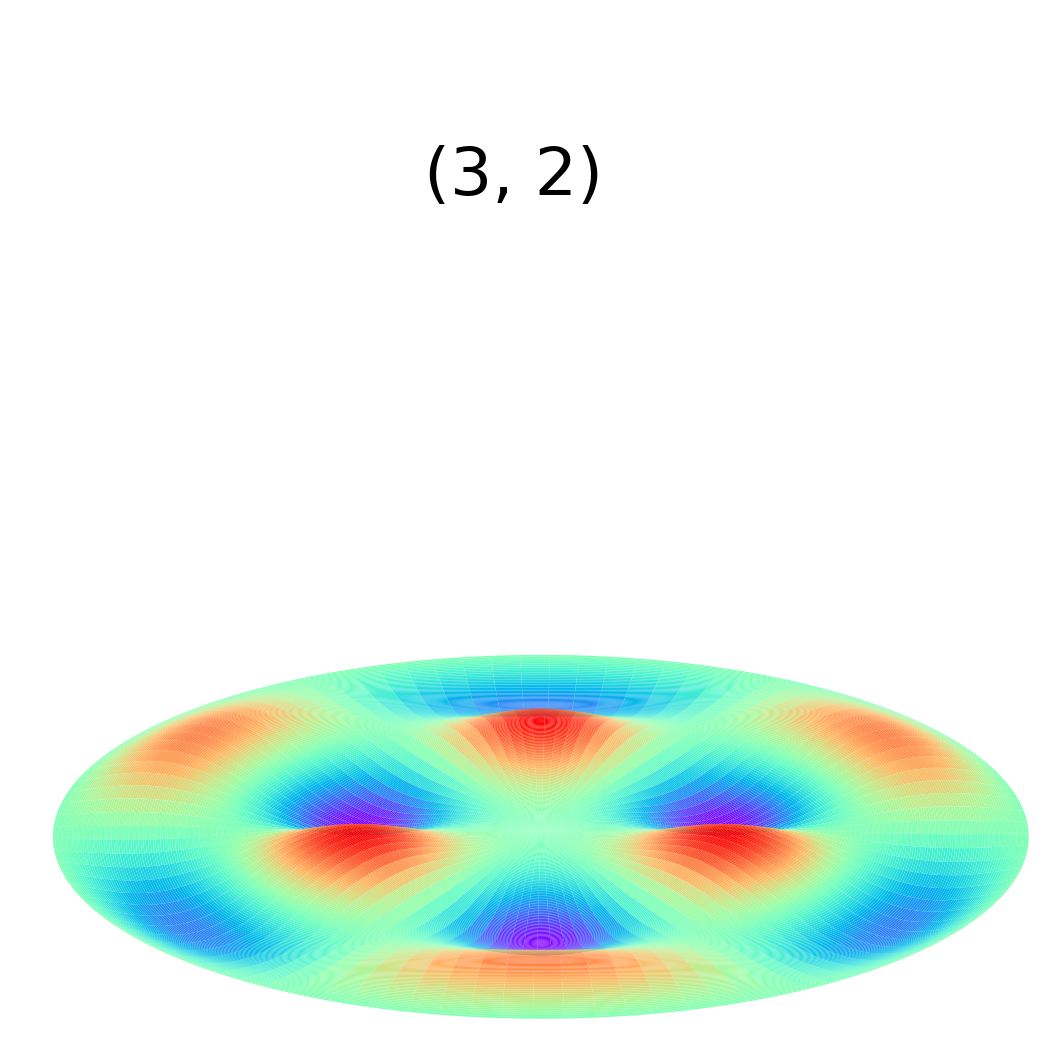
\includegraphics[scale=0.4]{3_2.png}
			& 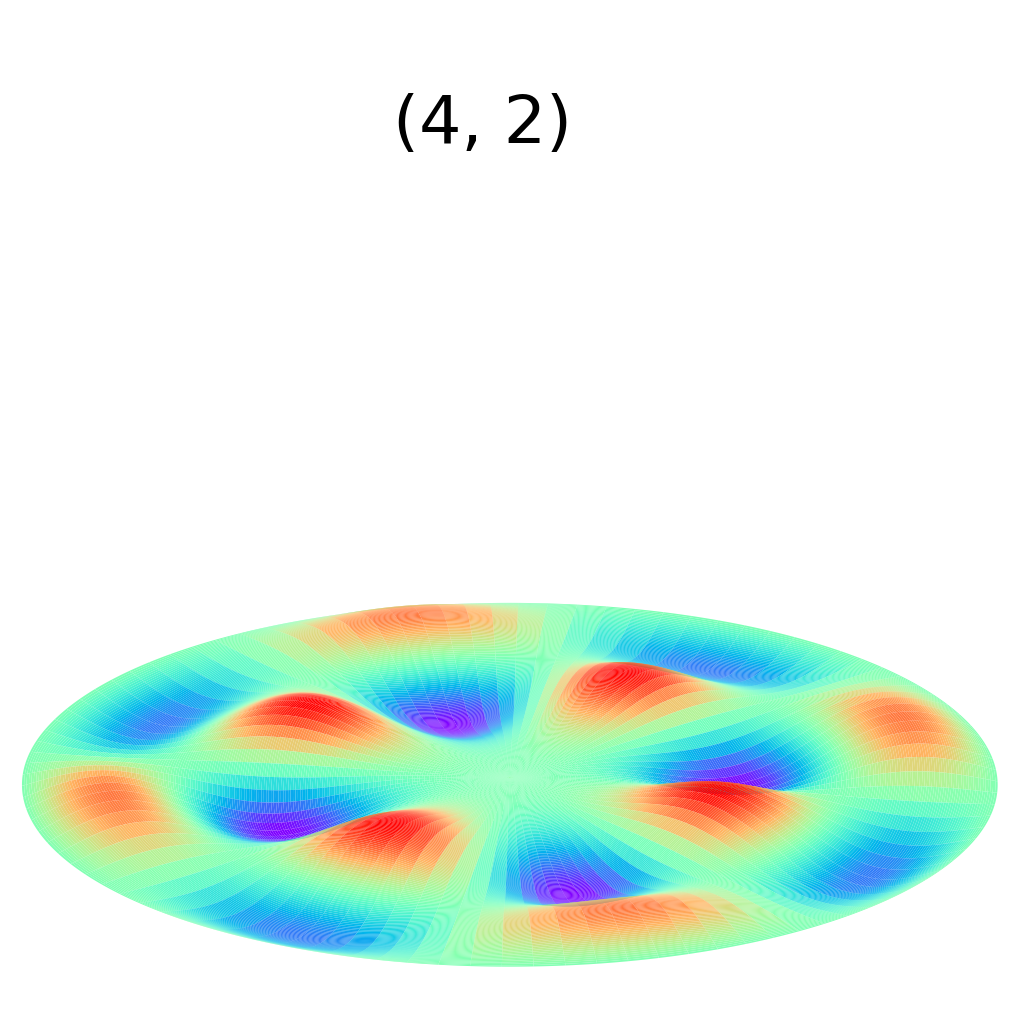
\includegraphics[scale=0.4]{4_2.png} \\
			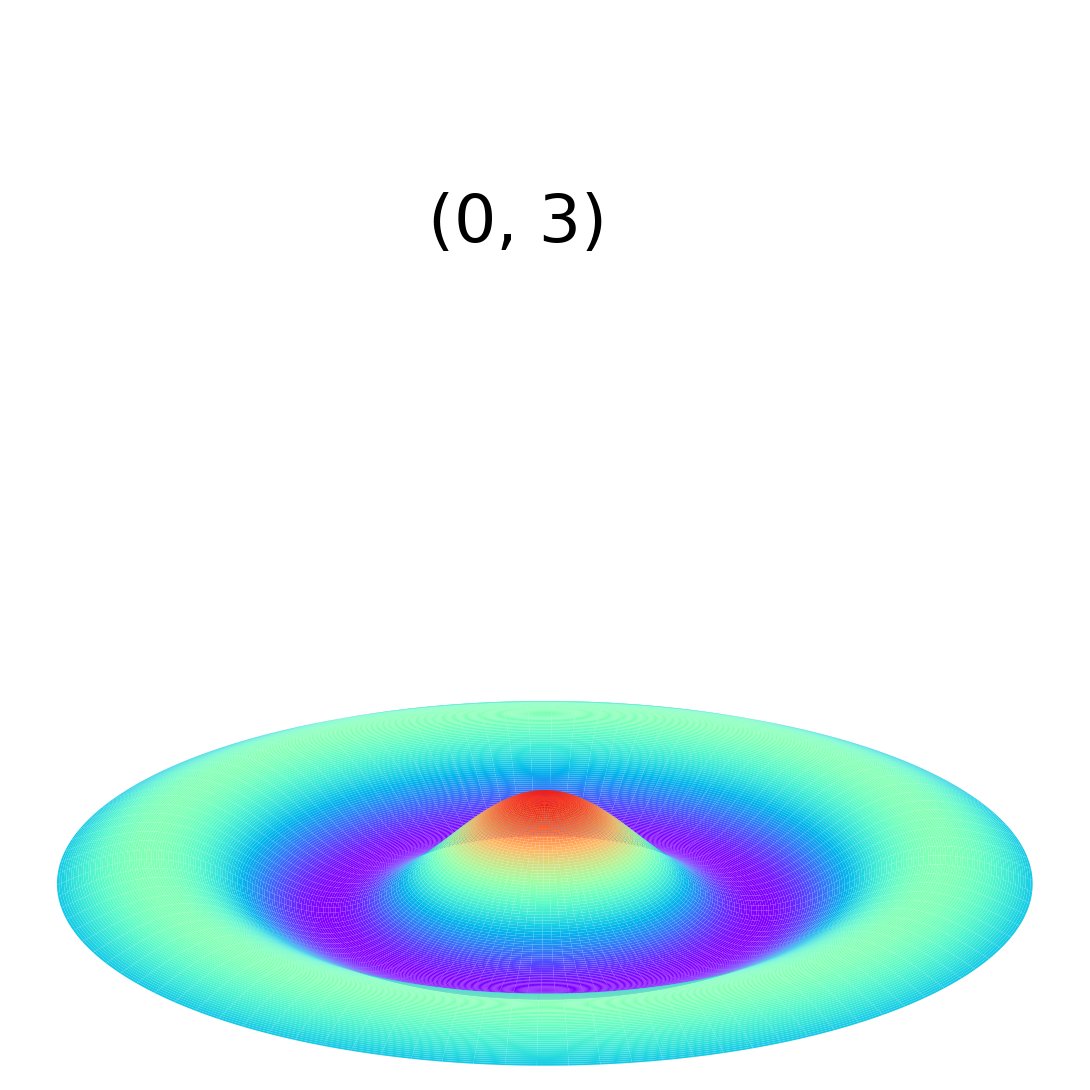
\includegraphics[scale=0.4]{0_3.png} & 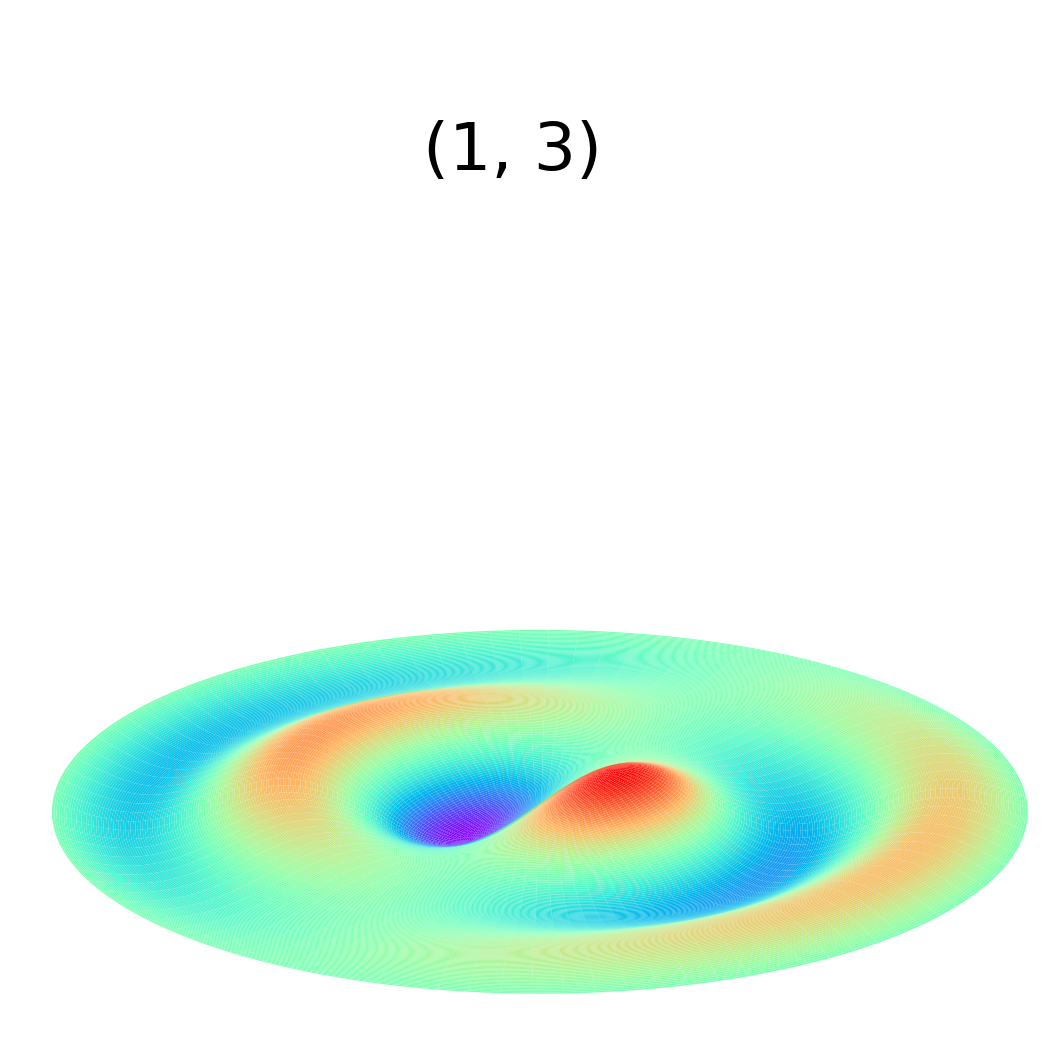
\includegraphics[scale=0.4]{1_3.png}
			& 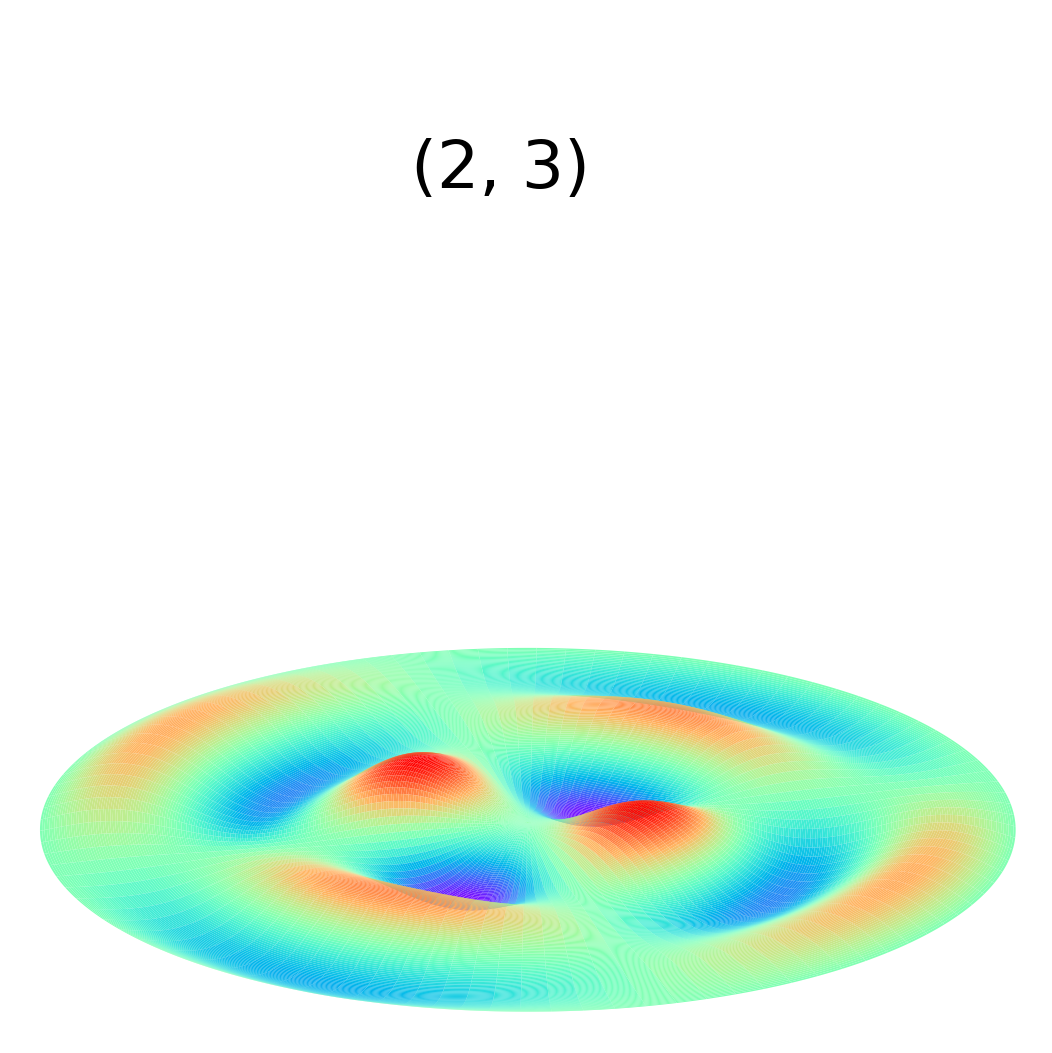
\includegraphics[scale=0.4]{2_3.png} & 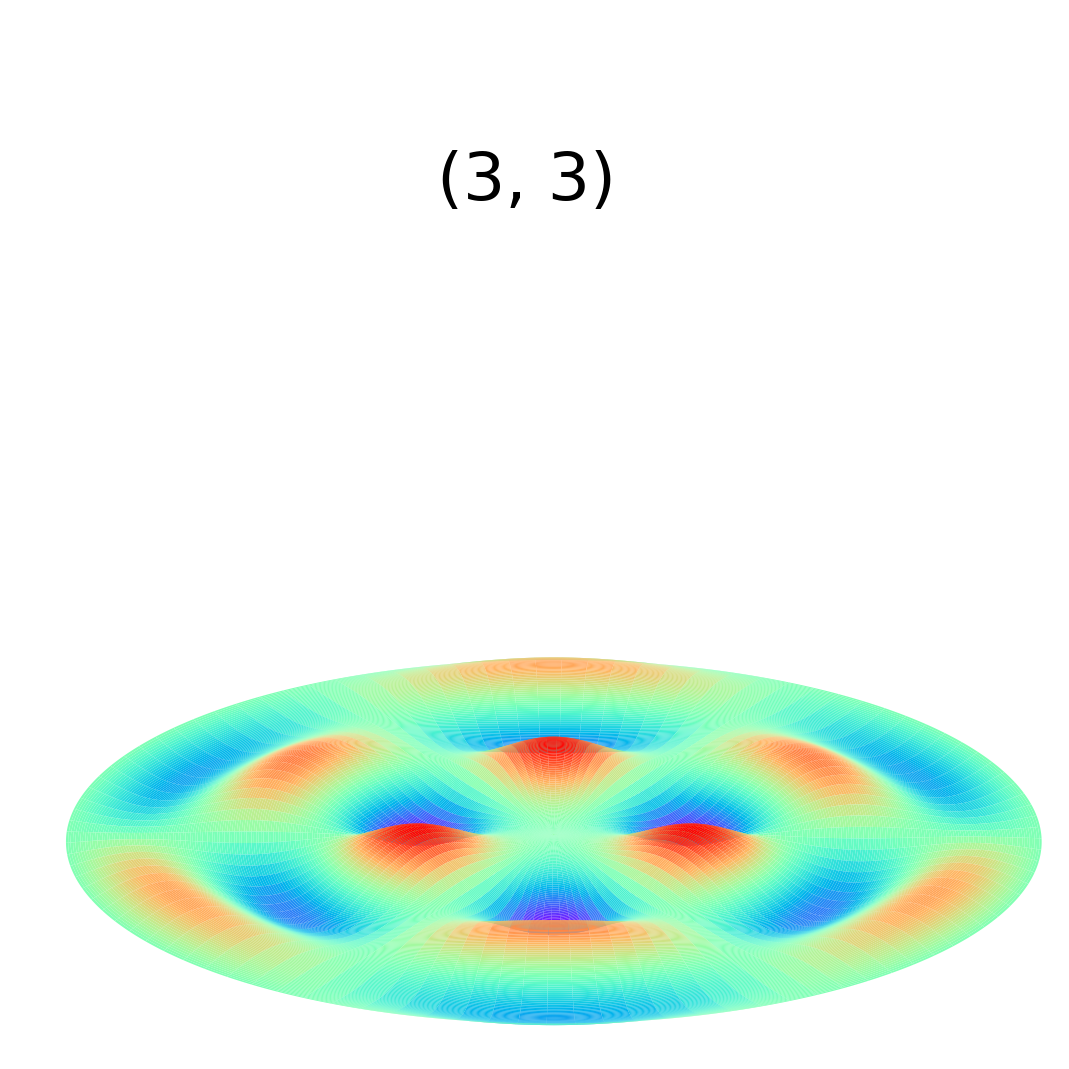
\includegraphics[scale=0.4]{3_3.png}
			& 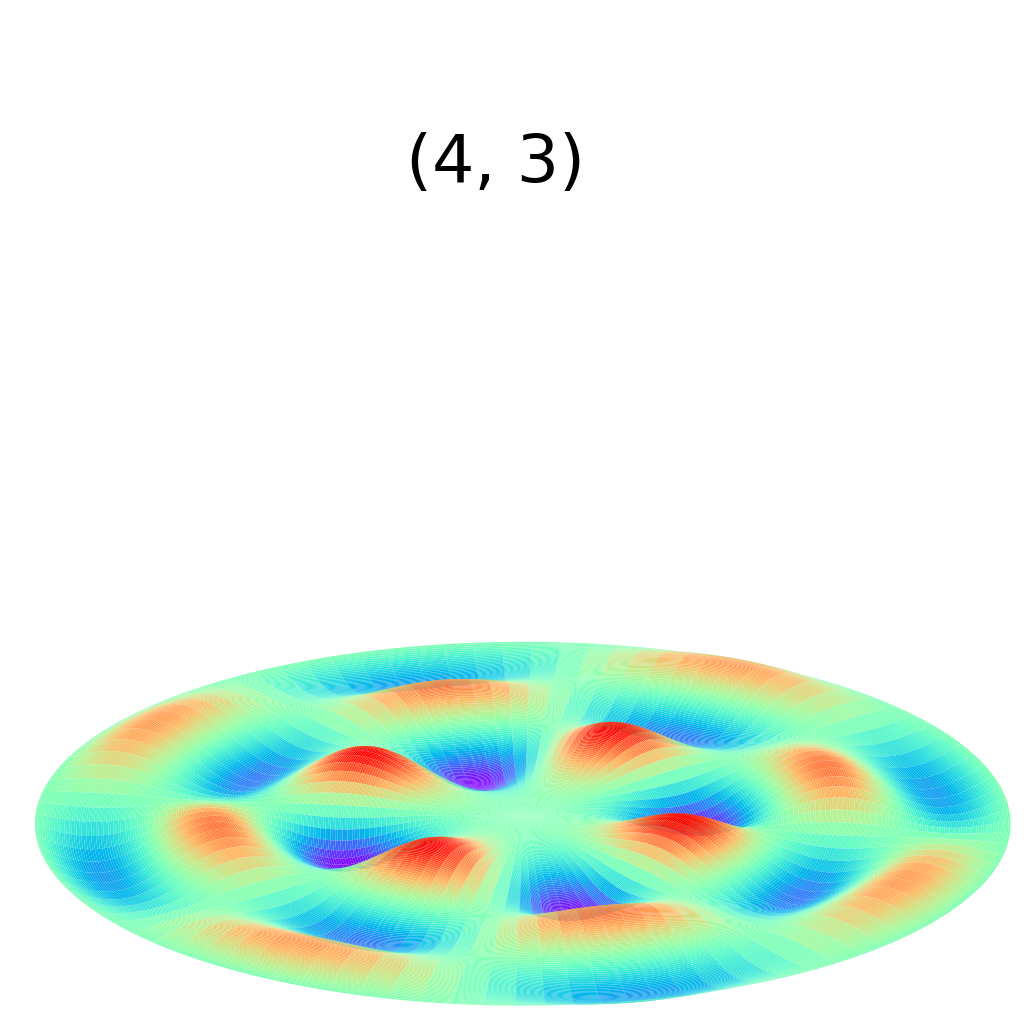
\includegraphics[scale=0.4]{4_3.png} \\
		\end{tabular}
		\centering 
		\caption{理想圆膜的振动模态}
		\label{visual mode}
	\end{figure}

	\subsection{真实圆膜的振动}
	\par 
	在构建波动方程(\ref{wave eq})时,只考虑了膜横向张力在法向的分力,但真实的
	薄膜在振动过程中应考虑空气阻力与膜的法向张力的影响。一般而言,空气阻力使薄膜振动
	模态的频率降低,而法向张力使薄膜振动模态的频率上升,但是对于\textbf{薄}膜,空气
	阻力的影响是最主要的\cite{phy_of_music}。
	\par 事实上空气阻力对于圆膜振动的影响非常复杂,应分为圆膜与自由空气的耦合、圆膜
	与封闭空气室耦合两种情况讨论。对于后者,圆膜具有圆柱对称性($m=0$)的振动模态
	会使得空气不断压缩与膨胀,这时空气压力会加快振动频率同时使振幅衰减很快,而$m>0$的
	振动模态只会使空气室内空气流动,不会压缩空气,这会使得所有非圆柱对称的振动模态
	频率降低;自由空气不会涉及到压缩与膨胀的问题,因而会降低所有振动模态的频率。
	\par
	考虑最简单的情况,空气阻力正比于膜振动的速度$\pdv{u}{t}$,将波动方程修改为:
	\begin{equation}
		\pdv{^2u}{t^2} = c^2\left[\pdv{^2u}{x^2} + \pdv{^2u}{y^2}\right] - 2b\pdv{u}{t}
	\end{equation}   
	仿照之前分离变量解方程的过程,可看出分离变量后空间部分的方程与[\ref{mode}]
	完全一致,而时间部分的方程变成了:
	\begin{equation}
		T_{mi}{''}(t) + 2bT_{mi}{'}(t) + c^2 \lambda_{mi} T_{mi}(t) = 0
	\end{equation}
	当阻尼足够小时($b^2 < c^2 \lambda$)这个方程的通解为:
	\begin{equation}
		T_{mi}(t) = A_{mi}\e^{-bt}\sin(\omega_{mi}{'}t + \phi_{mi})\quad\quad \omega_{mi}{'} = \sqrt{\left(\frac{c\mu_{i}^{(m)}}{a}\right)^2 - b^2}
	\end{equation}
	\par 从上面表达式可以看出,阻尼对于基频$\omega_{01}$的降低要比高频更加明显,即:
	\begin{equation}
		\frac{\omega_{mi}{'}}{\omega_{01}{'}} > \frac{\omega_{mi}}{\omega_{01}}\quad\quad \forall\, i > 1,\, m > 0
	\end{equation}                                                                                                                                                                                                                                                                                                                                                                                                                                                                                                                                                                                                                                                                                                                                                                                                                                                                                                                                                                                                                                                                                                                                                                                                                                                                                                                                                                                                                                                                                                                                                                                                                                                                                                                                                                                                                                                                                                                                                                                                                                                                                                                                                                                                                                                                                                                                                                                                                                                                                                                                                                                                                                                                                                                                                                                                                                                                                                                                                                                                                                                                                                                                                                                                                                                                                                                                                                                                                                                  
	\section{定音鼓的发声机制}
	\subsection{定音鼓的构造}
	\par 
	现代定音鼓以单面鼓为架构模式,由鼓皮、鼓身、鼓棰、定音系统等部分组成;
	鼓皮主要采用Mylar聚酯薄膜,相比于早先使用的牛皮,Mylar聚酯薄膜具有质地均匀、
	制作方便、受环境湿度影响小等优点。在实际应用中,厚度为0.19 mm的Mylar聚酯薄膜
	常作为定音鼓鼓皮的选用标准。定音鼓常采用铜作为鼓身材料,也常选用玻璃纤维等轻
	质材料。鼓身大致为半球形,末端留有小孔。
	\par 
	现代定音鼓的定音系统采用机械踏板调整螺栓的方法调节鼓面张力,
	代替了传统的需要手动调紧螺丝的设计。与传统定音鼓设计相比,
	采用踏板调节可以更快地调节定音鼓的音高,甚至可以让定音鼓产生滑音。
	\begin{figure}[htbp]
		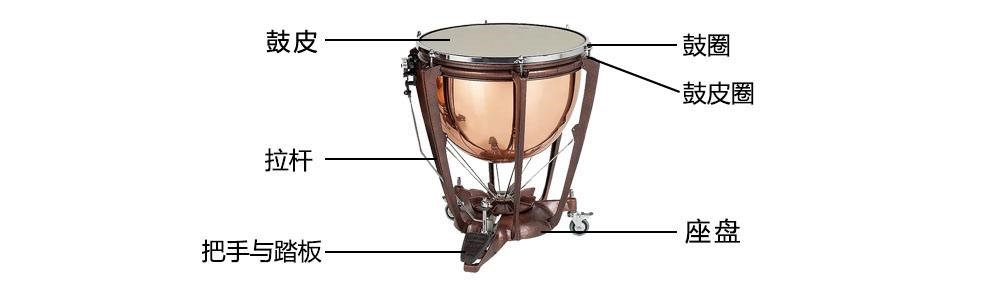
\includegraphics[scale=0.32]{timpani.jpg}
		\centering
		\caption{定音鼓的构造}
	\end{figure}
	\subsection{定音鼓的发声特点}
	\par 下面对于振动模态的标记采用与之前相同的记法。
    理想的二维薄膜振动与弦振动不同,其高次本征频率并不与基频成倍数关系。
	但经准确定音调节,定音鼓可以发出一个主音和至少两个与基频成倍数的泛音。
	Lord Rayleigh于1894年确定定音鼓的主音由(1,1)振动模态发出。后续的一些研究
	表明,定音鼓(1, 1)、(2, 1)、(3, 1)三个振动模态的频率比接近1 : 1.5 : 2。此外还
	发现(4, 1)和(5, 1)两个振动模态相比于(1, 1)振动模态的相对频率为2.44和2.90,
	可近似认为是2.50和3.00(2.44和2.90分别位于2.50和3.00对应的半个半音范围内)\cite{a}。
	因此,定音鼓主音和各级泛音的频率比约为2 : 3 : 4 : 5 : 6,这让定音鼓能够较好地表现出特定的音高。
	但但是对于理想圆膜,上述5个泛音频率比值应为2: 2.68 : 3.33 : 3.96 : 4.58。
	\subsection{定音鼓发出特定音高的原理}
	\par 
	上述理想二维圆形薄膜振动模态的相对频率比值为仅考虑无法向张力圆形薄膜自由振动得
	到的结果,但是定音鼓由于内部形成封闭的空气室因而必须考虑鼓面和空气室振动的耦合
	(可以参考本文之前的讨论),由于实际的膜具有厚度因而也会有法向张力对于振动的影响。
	理想比值与实际值(测量值)之间的差异可以认为是这两个因素导致的结果。
	\par 
	综合考虑定音鼓对应的物理模型,其能够发出特定音高的原理可以从以下四个方面进行考虑\cite{a}:
	\begin{itemize}
		\item[(1)]
		鼓面在空气介质中来回运动,导致主音对应的振动模态频率(即(1, 1)振动模态)
		相比理想情况有所降低,进而使得上述相对频率升高。
		\item[(2)]
		定音鼓内部的空气振动与鼓面振动可能会有相似的振动模态,并产生谐振。
		\item[(3)]
		定音鼓鼓面有一定的抗弯刚度,导致高次泛音对应的振动模态频率相比理想情况有所上升,
		进而使得泛音相对频率升高。
		\item[(4)]
		定音鼓鼓面有较大的剪切刚度。这导致鼓面会抵抗振动时产生的形变。
	\end{itemize}
	\par 
	研究表明,在上述四种可能的影响因素中,鼓内部空气运动带来的低频模态振动频率的下降与某些振动模态的缺失
	对定音鼓的音调性听感起到了决定性作用。其他因素带来的影响仅仅使频率产生了轻微的变化,
	或仅仅对音量的包络产生影响。
	\par 
	我们只讨论空气介质对频率造成的影响,因为这个因素对振动频率影响最大。由于薄膜振动
	会带动空气介质振动,可以假设该薄膜的质量相当于薄膜本身的质量加上一个空气负载的质量
	(薄膜振动会带动附近空气的振动)。
	对于一个半径趋于无穷的圆形活塞,其空气负载质量可以表示为:
	\begin{equation}
		m = \frac{\rho_{0}c_{a}\pi a^{2}X_1}{\omega}
		\label{air loading}
	\end{equation}
	\par 
	其中,$\rho_0$为空气密度,$c_a$为声速,$a$为活塞半径,$\omega$为活塞振动的圆频率,
	$X_1$为响应函数。对于频率$f < \frac{c_{a}}{4\pi a}$时,$X_1\approx\frac{16af}{3c_a}$;
	$f$处于高频时,$X_{1}~\frac{1}{f^2}$衰减。将负载质量与频率的关系图画出,
	如图(\ref{air loading p})所示,图中的实线是(\ref{air loading})式中计算出的结果,虚线为定音鼓薄膜的质量密度,
	作为参考使用。可以发现,对于频率越低的振动模态,其空气负载质量越大;而对于高频
	($f>500\mathrm{Hz}$)的频率,则几乎没有负载质量。已知:
	\begin{equation}
		\omega_{nk} = \frac{\mu_{k}^{(n)}}{a}\sqrt{\frac{\sigma}{\rho}}
		\label{frequency}
	\end{equation}
	空气的负载质量会使$\rho$增大,最终的结果导致$\omega$降低,并且对频率越低的振动模态,
	其频率的相对降低越严重,导致泛音列频率比值上升,与实验值定性上相吻合。
	\begin{figure}[htbp]
		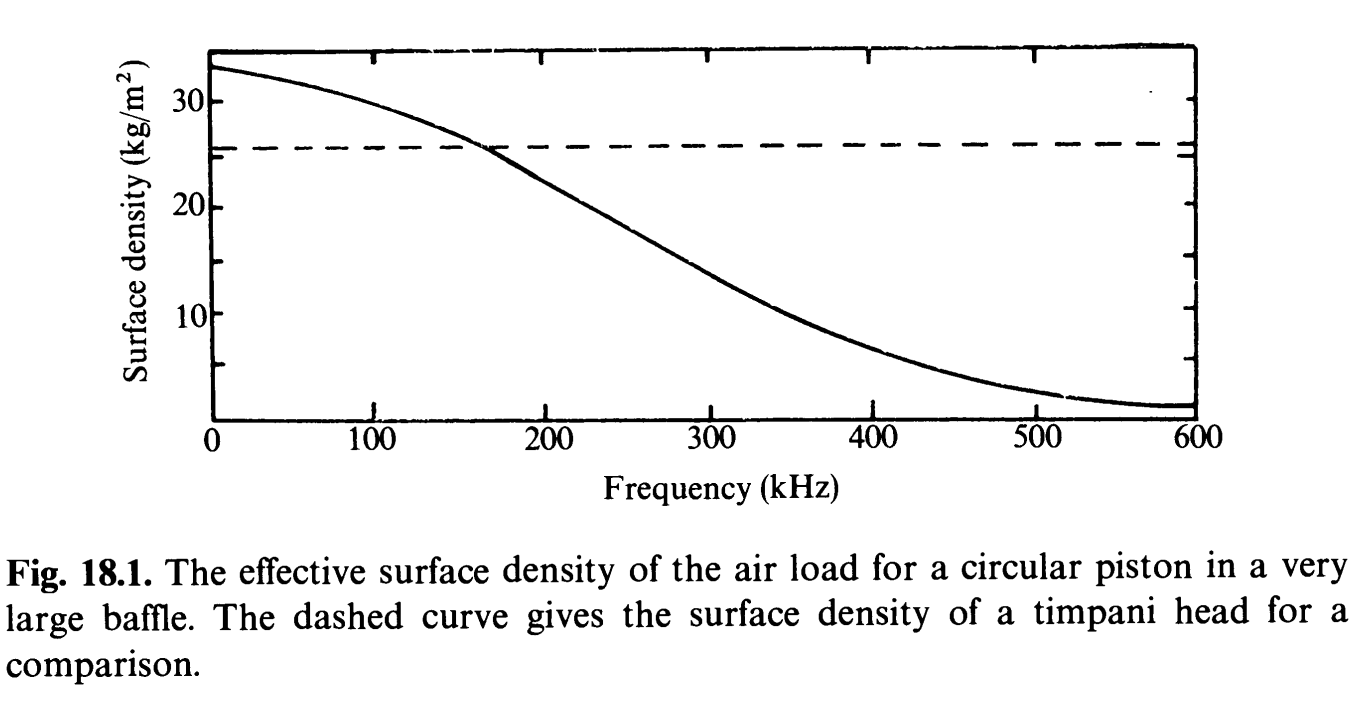
\includegraphics[scale=0.32]{effective_mass.png}
		\centering 
		\caption{空气负载质量与频率的关系\cite{a}}
		\label{air loading p}
	\end{figure}
	\par 
	在上面的假设下只能进行定性的分析,更精确的计算必须考虑空气振动与薄膜振动的耦合
	,可以通过格林函数法来求解这样一个耦合系统波动方程的振动模态,其计算结果
	与实验值几乎没有差别\cite{Christian1984Effects}。由格林函数精确计算的
	数据由表(\ref{calculate fre})给出。从表中可以看出,即使是只有薄膜在空气中振动而没有定音鼓桶的
	情况下,其(1, 1)、(2, 1)、(3, 1)、(4, 1)、(5, 1)的频率比已经非常接近于
	2 : 3 : 4 : 5 : 6。另外注意到表(\ref{calculate fre})中(0, 1)模态在有鼓桶和无鼓桶
	时频率的较大差别,这可以定性解释为,(0, 1)对应的鼓面振动模态涉及到对鼓内空气的压缩
	和膨胀,相当于给鼓面增加了一个沿振动方向的力,从(\ref{frequency})式中看,这导致σ增大
	从而导致(0, 1)模态的振动频率在有鼓桶时明显高于没有鼓桶的情况。
	\begin{figure}[htbp]
		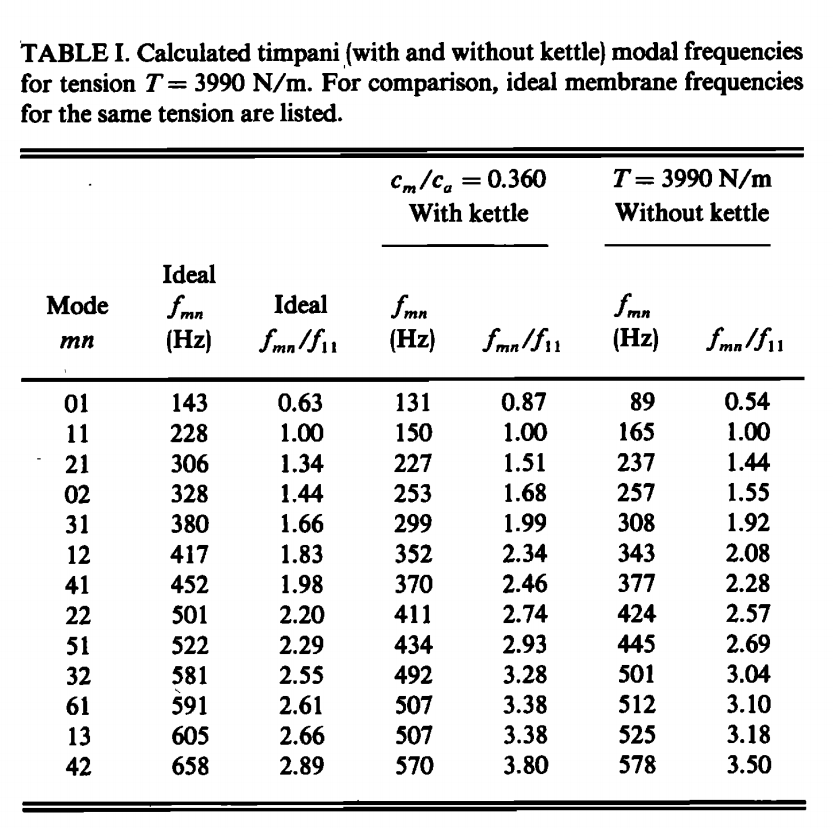
\includegraphics[scale=0.4]{calculate_frequency.png}
		\centering
		\caption{理论计算的真实鼓面振动与理想圆膜振动的频率差异\cite{Christian1984Effects}}
		\label{calculate fre}
	\end{figure}
	\par 
	以上从物理模型的角度分析了定音鼓够发出特定音高的原理,接下来简述上述频率比为连续整数
	的主音和泛音列传入人耳形成固定音高的原理。根据基频缺失效应(missing fundamental effect),
	人耳感觉到的基频音高会偏向于泛音列的最大公约数。例如:从A4出发的纯五度音,泛音列是440、660、880……,
	有最大公约数,因此可以很好地听出音高感。因此对于上述定音鼓主音和泛音列,
	其频率比为2 : 3 : 4 : 5 : 6,有最大公约数1,可以听出相对频率为1的音高。
	\section{有固定音高乐器与无固定音高乐器}
	\subsection{概述}
	\par 
	一般来说,打击乐器可以分为两类,一类是具有固定音高的(definitely pitched),另一类是无固定音高的
	(indefinitely pitched或unpitched)。顾名思义,固定音高的乐器在演奏中发出的声音可以被人耳分辨出
	确定的音高,而无固定音高的乐器发出的声音尽管也有特定的频率特征,但在人耳听来却难以分辨出一个确定的音高。
	\par 
	前面讨论过的定音鼓,以及木琴之类的打击乐器是固定音高的;而一般的鼓、钹、镲则属于无固定音高的打击乐器。
	在通常情况下,非固定音高乐器由于没有固定的音高,与音乐的旋律没有直接的关系,因此其主要作用是节奏强调。
	在管弦乐中,这部分打击乐通常被称为辅助打击乐。
	\subsection{固定音高和非固定音高的基本特征}
	\par 
	在之前关于定音鼓的讨论中,我们已经了解到,如果一种声音的基音与泛音列的频率可以形成(简单)整数比
	(这样声音的波形就有周期性),则它可以被人耳分辨出固定音高。相反,如果一种声音缺乏这种固定音高的性质,
	它就无法被分辨出固定音高。
	\par
	一般来说,非固定音高的声音有两种情况。一种情况便是声音的基音和泛音的频率不能形成整数比,
	因而不能被听出固定音高。而在另一种情况中,声音的频谱中根本没有一个强度足够大的基频,而是在一定的频率范围内,
	各种频率的强度基本相仿,即声音接近于一定频率范围内的白噪声,这样的声音显然也不能被分辨出固定音高。
	\par
	无论是上述的哪一种情况,非固定音高的声音都不具备周期性的波形,属于物理上的“噪音”,然而,
	非固定音高的乐器在音乐实践中有重要的作用。因此,我们必须注意到,音乐中的声音并不仅仅包含有固定音高的乐音,
	也包含着不可或缺的“噪音”成分。
	\subsection{固定音高和非固定音高乐器的区别与关系}
	\par 
	通过上面的讨论,我们可以给出固定音高乐器和非固定音高乐器最简单、最基本的区别,也就是它们发出的声音的性质不同。
	固定音高乐器发出的声音的基音和泛音列的频率可以形成(简单)整数比,具有周期性的波形;而非固定音高乐器则与之相反,
	发出没有周期性波形的“噪音”。
	\par
	而这些乐器之所以会发出不同性质的声音,则与它们的物理性质和发生原理相关。课上已经介绍过一维弦的振动问题的简单求解,
	而前文中我们也讨论了二维圆膜振动问题的求解。从两种情况的解中,我们可以看出,(都是在最简单的情况下)一维弦振动发
	出的声音的基音与泛音列符合简单整数比,而二维圆膜振动发出的声音的基音和泛音的频率比则不是整数比。这可以解释,
	弦鸣乐器通常都是固定音高的,而一般的膜鸣乐器(如一般的鼓)则通常是非固定音高的。
	\par 
	而事实上,固定音高乐器与非固定音高乐器之间并没有不可逾越的鸿沟。事实上,我们可以通过一些手段改变乐器的发声性质,
	从而在某种程度上实现两者的转换。一般的鼓是非固定音高乐器,但通过特定的演奏方法,或者改变其某些部件的结构,
	可以设法使其发出声音中有整数比关系的一部分泛音得到突出,或者使其声音的泛音列频率比更接近于整数比,从而使其接近于固定音高乐器
	(参考定音鼓部分)。钢琴等弦鸣乐器是固定音高乐器,但如果在其琴弦处放置某些物品来破坏其泛音列的整数比性质,
	则也可以使其成为非固定音高乐器(即所谓“加料钢琴”)。
	\section{致谢}
	感谢每一位参与作业的小组成员:
	\begin{itemize}
		\item 王崇斌\,\,1800011716\,\,化学与分子工程学院
		\item 陆浩成\,\,1800011742\,\,化学与分子工程学院
		\item 任熠辰\,\,1800012194\,\,生命科学学院
		\item 李恒宇\,\,1900011794\,\,化学与分子工程学院
		\item 鲁承浩\,\,1900011828\,\,化学与分子工程学院
		\item 昌珺涵\,\,1700011741\,\,化学与分子工程学院
	\end{itemize}
	\bibliographystyle{unsrt}
	\bibliography{ref}
\end{document}
